\documentclass{article}
\usepackage{amsmath}
\usepackage{amsfonts}
\usepackage{graphicx}
\usepackage{geometry}
\usepackage{bm}
\geometry{top=2.5cm,left=2.5cm,right=2.5cm,bottom=2.5cm}
\title{Progress on Simulation}
\author{}
\date{}
\begin{document}
\maketitle

\section{The distribution of the result of estimation}
The boxplots and quantile plots for the result can be seen in the following figures. From the further result of how median and variance changed with epsilon, I choose larger epsilon from 0.1-0.5. And the distributions are similar for epsilon in this range, I select and  epsilon = 0.35 for the case n = 1000 and epsilon = 0.15 when n = 4000 as typical examples. The result shows that in both these cases, the estimation is very sensitive to noise and only approximately 30\% of the result will lie in area with 50\% relative error compared to the true value. Also very large result does occur with relatively low probabibility. 
\begin{figure}[htbp]
\centering
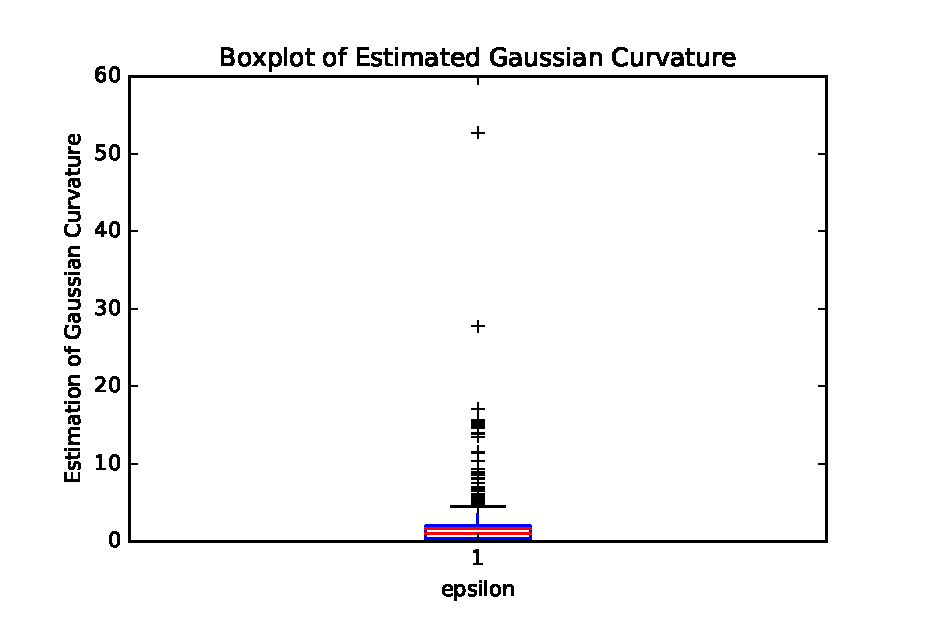
\includegraphics[width=0.8\textwidth]{Boxplot-size-1000-epsilon-35.eps}
\caption{Boxplot of estimated Gaussian curvature,red line below is the mean value 1.70, and orange line lower of median is 0.99}
\label{bp1000}
\end{figure}

\begin{figure}[htbp]
\centering
\begin{minipage}{0.45\textwidth}
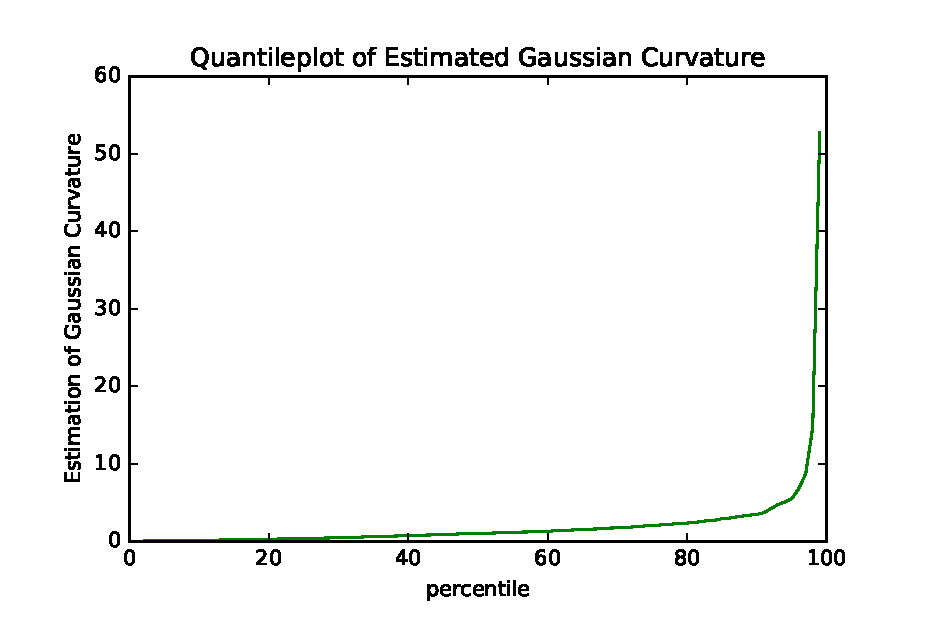
\includegraphics[width=0.9\textwidth]{Quantileplot-size-1000-epsilon-35.eps}
\caption{Quantile plot (Full) for estimation result}
\label{qp1000}
\end{minipage}
\begin{minipage}{0.45\textwidth}
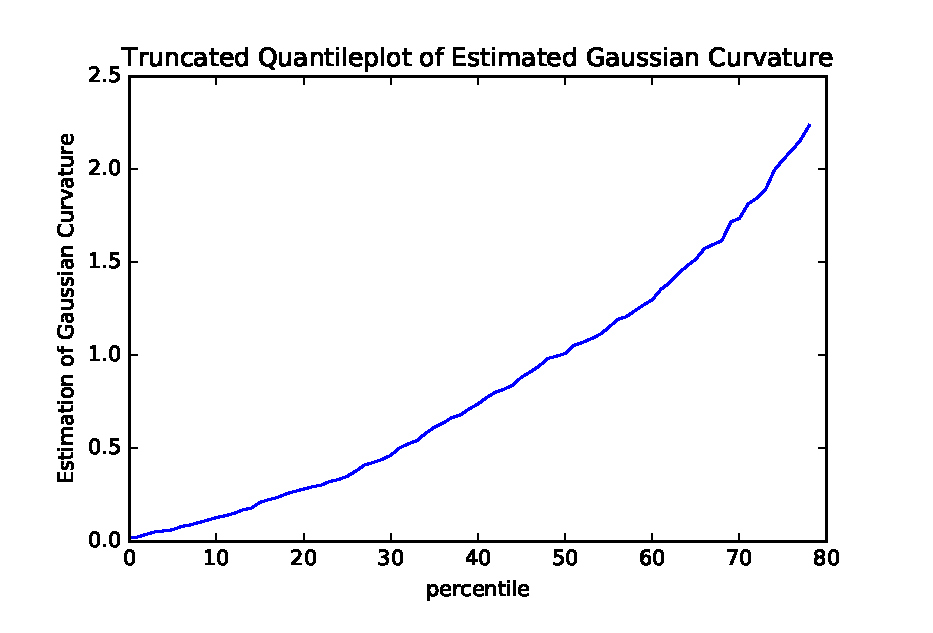
\includegraphics[width=0.9\textwidth]{Trun-Quantileplot-size-1000-epsilon-35.eps}
\caption{Truncated quantile (from 0 to 80\%) plot for estimation result}
\label{tqp1000}
\end{minipage}
\end{figure}

\begin{figure}[htbp]
\centering
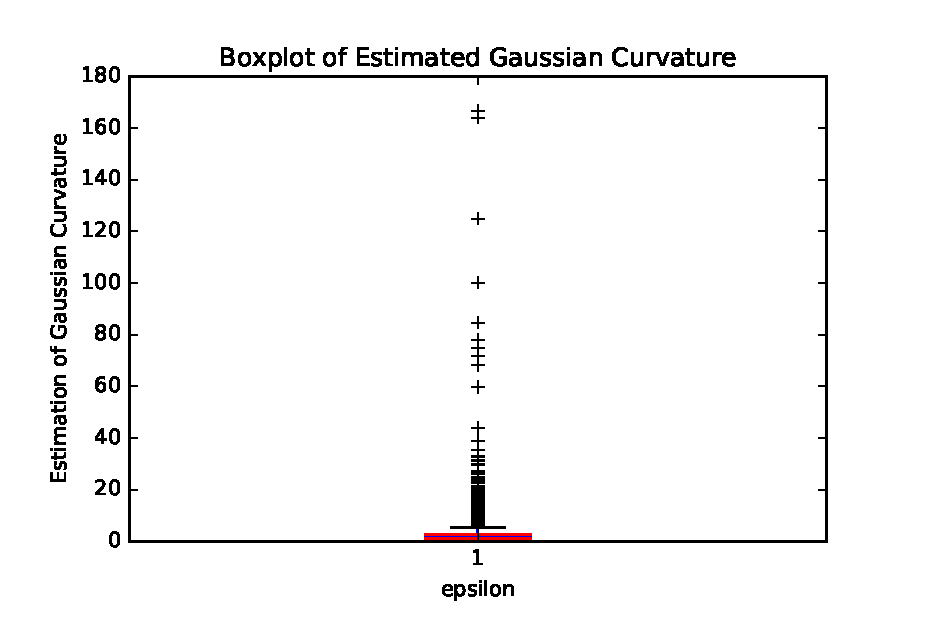
\includegraphics[width=0.8\textwidth]{Boxplot-size-4000-epsilon-15.eps}
\caption{Boxplot of estimated Gaussian curvature,red line below is the mean value 2.74, and median line is lower at 1.10}
\label{bp4000}
\end{figure}

\begin{figure}[htbp]
\centering
\begin{minipage}{0.45\textwidth}
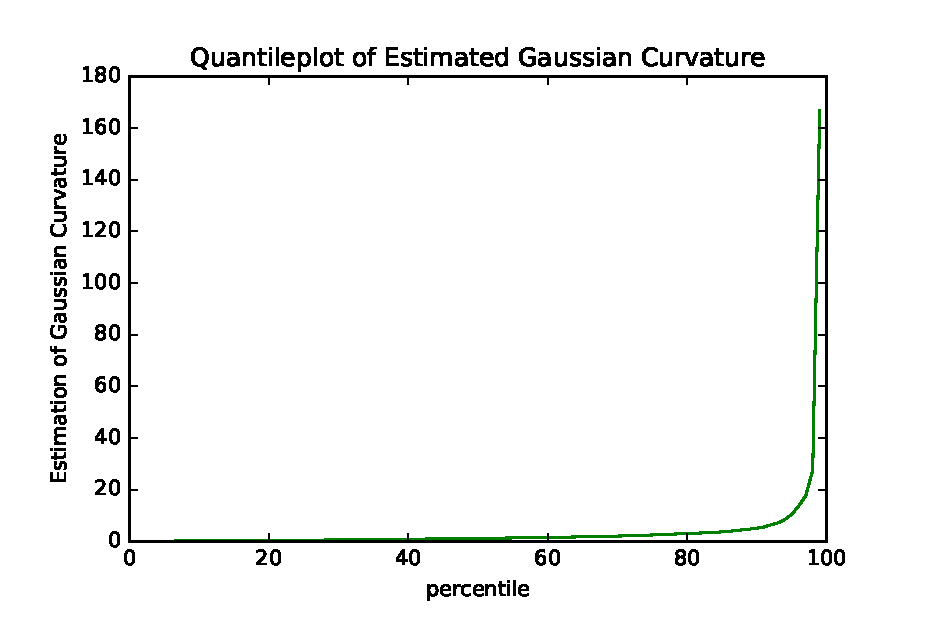
\includegraphics[width=0.9\textwidth]{Quantileplot-size-4000-epsilon-15.eps}
\caption{Quantile plot (Full) for estimation result}
\label{qp4000}
\end{minipage}
\begin{minipage}{0.45\textwidth}
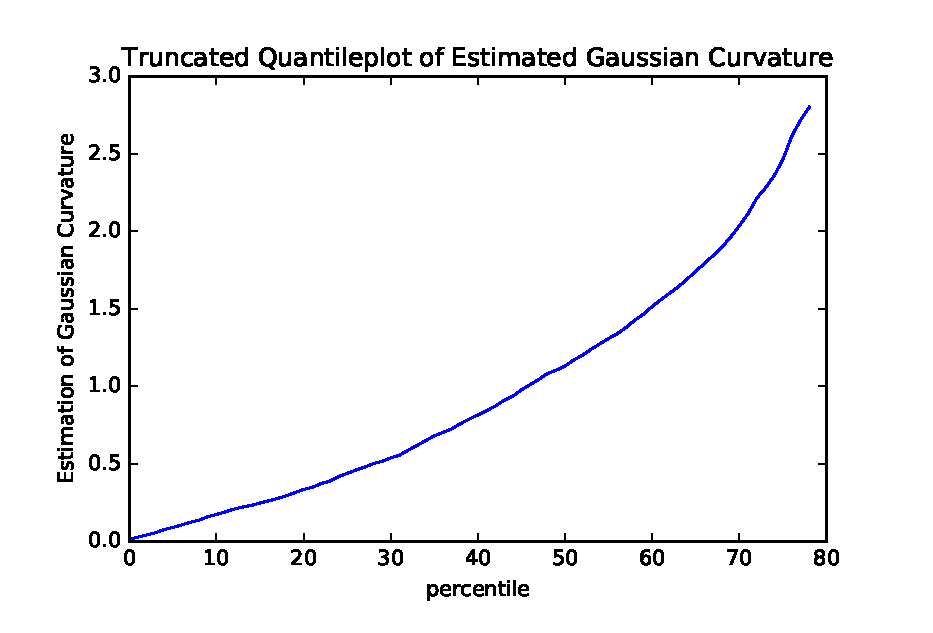
\includegraphics[width=0.9\textwidth]{Trun-Quantileplot-size-4000-epsilon-15.eps}
\caption{Truncated quantile (from 0 to 80\%) plot for estimation result}
\label{tqp4000}
\end{minipage}
\end{figure}
The result reveals that the estimation result may not concentrate around the true value. The median of the results will be cose to the true value while the mean may have a big bias due to the enormous data. 

\newpage
\section{Local PCA}
In this part I conduct experiments to see how local PCA contributes to the errors of our estimation of Gaussian curvature. I did this from in following perspectives:
\begin{enumerate}
\item I compared the estimated local PCA basis with the true basis. Suppose $\widehat{O}=(\bm{u}_1,\bm{u}_2)$ is the estimated basis of tangent space and $O_{true}$ is the true tangent space. For any data point $(x_0,y_0,z_0)$ on the sphere, the true tangent space is a plane with normal vector $(x_0,y_0,z_0)$. And the estimated tangent plane has a normal vector $\bm{n}=\bm{u}_1\times \bm{u}_2$. To see the difference between the estimated tangent plane, we would only need to calculate the cosine between the two normal vectors. 
\item We can calculate that a basis for the true tangent plane at point $(x_0= r \cos \theta \cos \phi,y_0 = r \cos \theta \sin \phi, z_0 = r\sin \theta)$ is normalized vector of $(-r\sin \theta \cos \phi, -r \sin \theta \sin \phi, r \cos \theta)$ and $(-r \cos \theta \sin \phi, r \cos \theta \cos \phi, r \cos \theta)$ we can calculate the orthonormal matrix $O$ that is closest to $\widehat{O}^TO_{true}$ in the sense of Hilbert-Schmidt norm and calculate the norm to show how close the two tangent planes are. More formally, we find 
\begin{equation}
	O = \arg\min_{O\in O(d)}\parallel O-\widehat{O}^TO_{true} \parallel_{HS}
\end{equation}
where $\parallel A \parallel_{HS}=\text{tr}(AA^T)$
\item From two basis of the tangent plane $\widehat{O}$ and $O_{true}$ we can calculate the $O_{pq}$ matrices which approximate the parallel transport operator from both sets of basis and further calculate the Gaussian curvature. 
\end{enumerate}
The result can be shown in figure, we show the result of epsilon = 0.35 for size = 1000 and epsilon = 0.15 for size = 4000, since the results are similar.

\begin{figure}[htbp]
\centering
\begin{minipage}{0.45\textwidth}
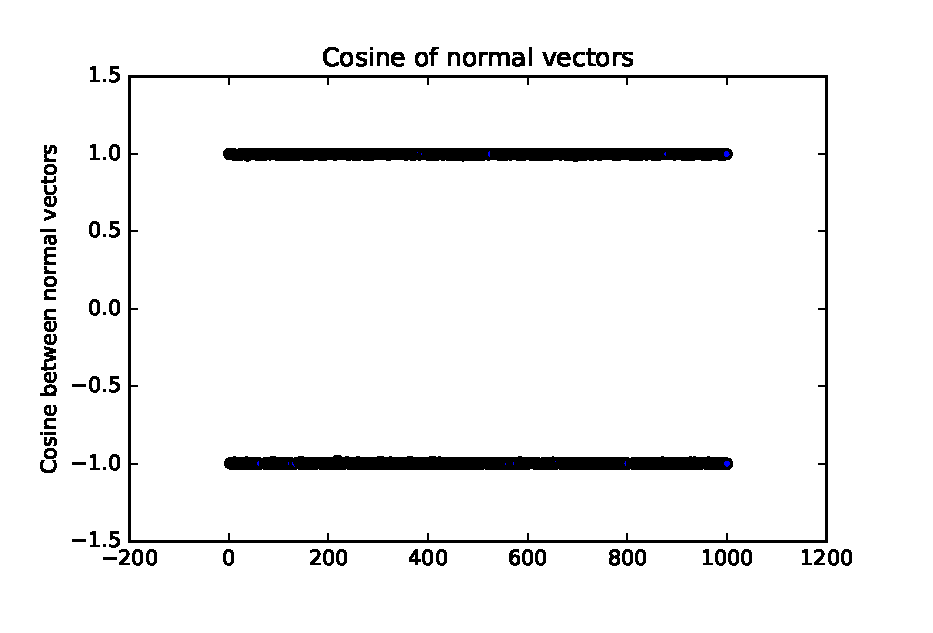
\includegraphics[width=0.9\textwidth]{Normcos-size-1000.eps}
\caption{Cosine of norm vectors, size = 1000}
\label{normcos1000}
\end{minipage}
\begin{minipage}{0.45\textwidth}
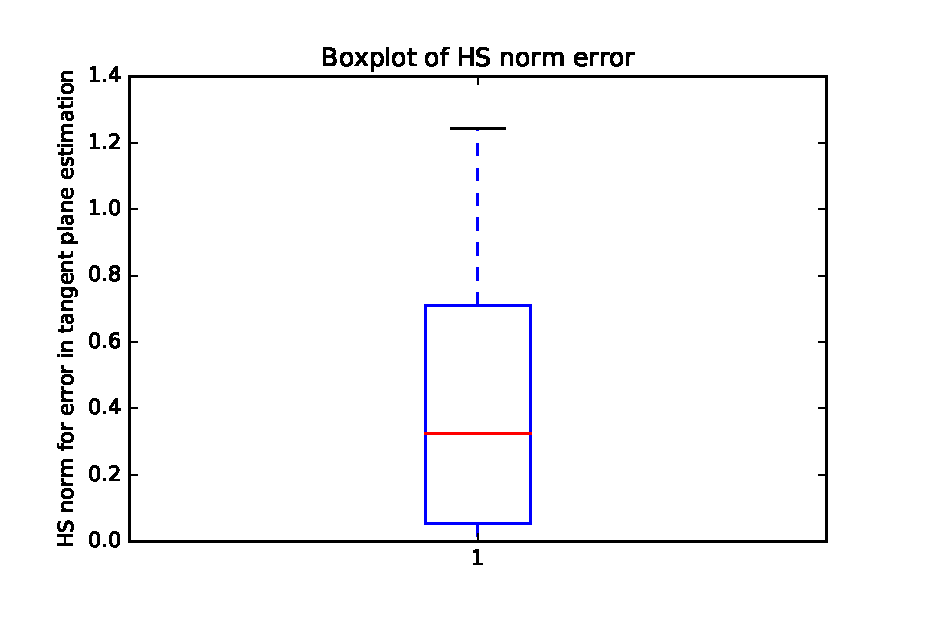
\includegraphics[width=0.9\textwidth]{HSlpca-size-1000.eps}
\caption{HS norm between estimated tangent plane and true tangent plane, size = 1000}
\label{hsnorm1000}
\end{minipage}
\end{figure}

\begin{figure}[htbp]
\centering
\begin{minipage}{0.45\textwidth}
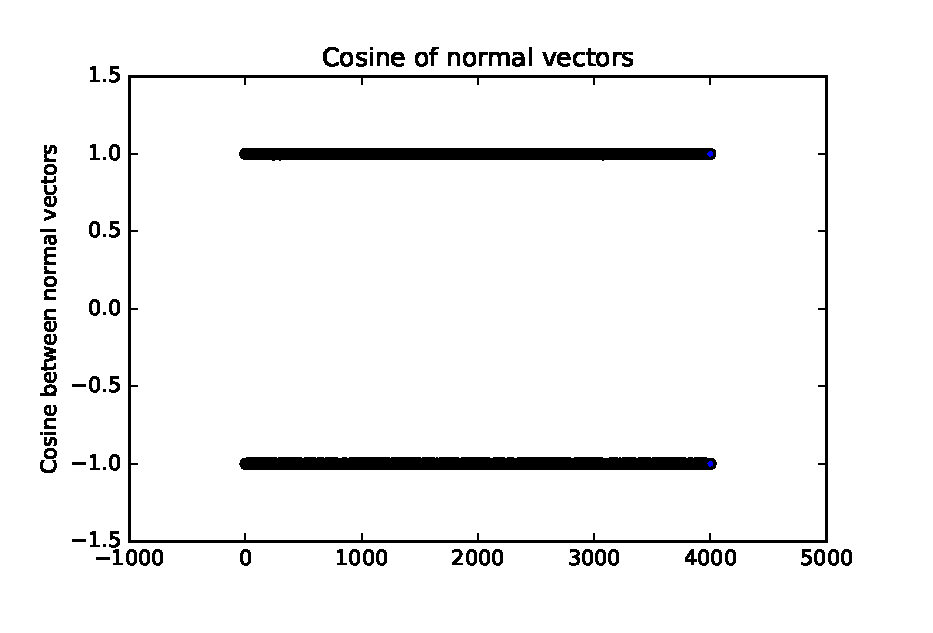
\includegraphics[width=0.9\textwidth]{Normcos-size-4000.eps}
\caption{Cosine of norm vectors, size = 4000}
\label{normcos4000}
\end{minipage}
\begin{minipage}{0.45\textwidth}
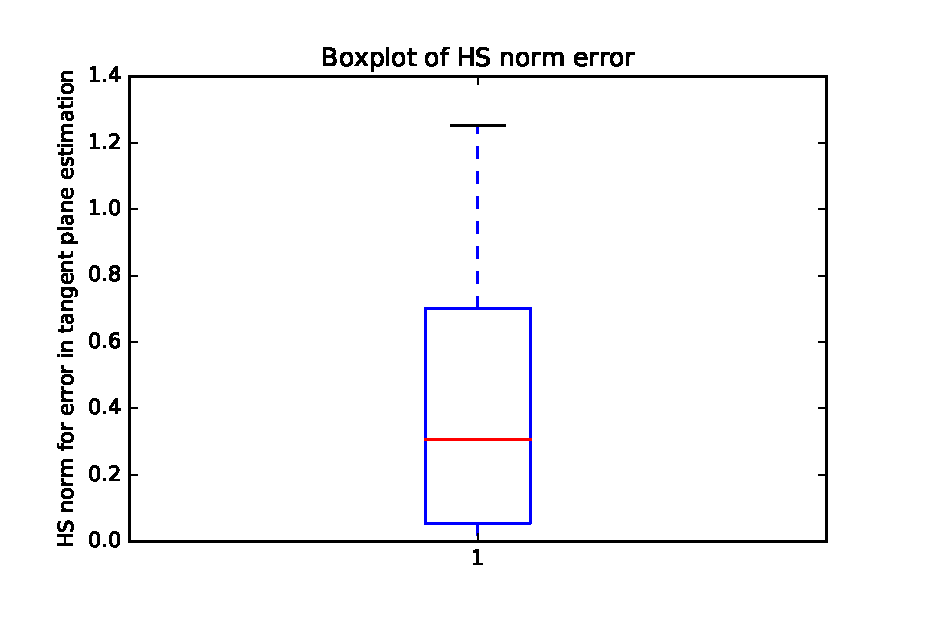
\includegraphics[width=0.9\textwidth]{HSlpca-size-4000.eps}
\caption{HS norm between estimated tangent plane and true tangent plane, size = 4000}
\label{hsnorm4000}
\end{minipage}
\end{figure}
From the results we can see that the estimation of tangent plane can be regarded as reliable. As the figure of cosine between estimated normal vector shows that the normal vector of the estimated tangent plane is close to the true normal vector, in the sense that  they lie in the same striaght line. The different signs of cosines between normal vectors is due to the orientation of local basis. And the HS norm distribution shows that they are quite close to the real tangent plane.
\par
Also with the true tangent plane I calculated the estimation of Gaussian curvature. The result is almost the same as the one calculated after local PCA tangent plane. This also shows that the mean variance comes from the calculation of curvature itself.
\end{document}